\section{The Discrete Uniform Distribution, PDFs and CDFs}\label{sec2:discreteuni}

In this section we consider probability distributions and how to sample them on a computer.\footnote{For further reading on probability distributions, see \cite{larsenmarx2004}.}
The \textbf{probability} of an event is a measure of how likely that event will occur, it can be understood as the ratio of the number of ways it can occur to the entire space of possible outcomes.
\textbf{Probability distributions} contain information about the probabilities of different possible outcomes in an experiment.
In the next example we define two important probability functions.

\begin{myexample}\label{2_dice_example}
Consider the experiment of rolling a fair six-sided die with the numbers 1 to 6 on its faces.
Each face has an equal chance of coming up when the die is rolled -- so the probability that we get the number 1 (e.g.) is $\frac{1}{6}$.
Using $X$ to denote the random variable representing the outcome of this experiment, we can state this as $P(X = 1) = \frac{1}{6}$. Similarly, $P(X = 2) = \frac{1}{6} = P(X = 3) = \cdots$.

\begin{figure}[htbp]
	\centering
	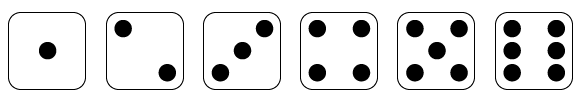
\includegraphics[width=0.6\textwidth]{fig/2_dice_example.png}
	\caption{Each outcome has equal probability $= \frac{1}{6}$. \label{fig:2_dice_example}}
\end{figure}


The probability distribution for $X$ assigns a probability of $\frac{1}{6}$ to each of the six possible outcomes -- this is the \emph{uniform distribution} from Section~\ref{sec1} applied to the integers $\{1,2,\ldots,6\}$. 
We can capture this information concisely using a \textbf{probability density function}, or a \textbf{pdf}.
This is a function $f(k)$ that takes as input the outcome $k$, and outputs the probability that $X = k$.
That is, the pdf for the random variable $X$ is \[ f(k) = P(X = k) = \left\{ \begin{matrix} \frac{1}{6}, & k = 1,2,\ldots, 6 \cr 0, & \text{ otherwise.} \end{matrix} \right. \]


Recall from Section~\ref{sec1} that we call this a uniform distribution, since each outcome is equally likely.
In particular, $X$ is said to have a \textbf{discrete uniform distribution}, since there are only a finite number of possible outcomes.

We also define the \textbf{cumulative distribution function} of a random variable, also called its \textbf{cdf}.
As the name suggests, this function $g(k)$ takes as input an outcome $k$, and outputs the probability that $X \leq k$; that is, $g(k) = P(X \leq k)$.
For this example, the cdf of $X$ is \[ g(k) = P(X \leq k) = \frac{\lfloor k \rfloor}{6}, \ k = 1,2,\ldots,6. \qed \] 

\begin{figure}[htbp]
 \begin{minipage}{.5\textwidth}
        \centering
	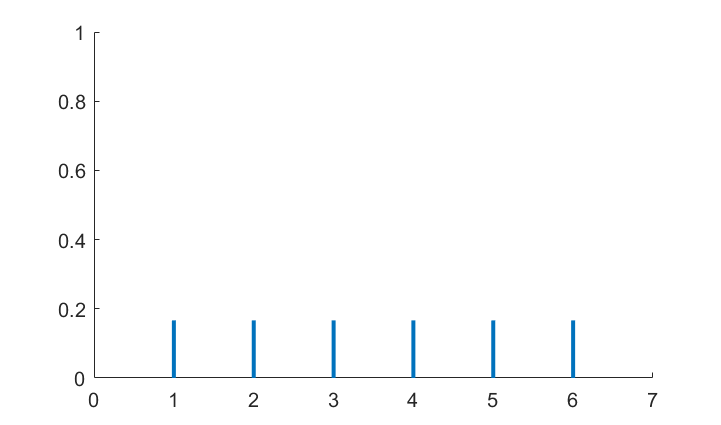
\includegraphics[width=0.9\linewidth]{fig/2_dice_pdf}
    \end{minipage}
    \begin{minipage}{0.5\textwidth}
        \centering
	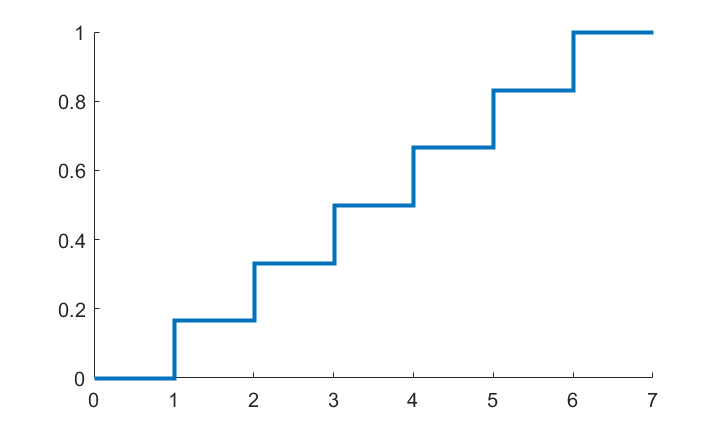
\includegraphics[width=0.9\linewidth]{fig/2_dice_cdf}
    \end{minipage}	
    \caption{The pdf (L) and cdf (R) of $X$\label{fig:2_dice_pdf}}
\end{figure}


\end{myexample}

In general, given a finite set of outcomes $S = \{a,a + 1,\ldots,b\}$, with $n = |S| = b-a+1$, the discrete uniform distribution over this set has pdf \[ f(k) = \left\{ \begin{matrix} \frac{1}{n}, & k \in S \cr 0, & \text{ otherwise.} \end{matrix} \right.\]
while its cdf is \[ g(k) = \left\{ \begin{matrix} 0, & k < a \cr \lfloor \frac{k - a + 1}{b - a + 1} \rfloor, & a \leq k \leq b \cr 1, & k > b \end{matrix} \right. \]
If a random variable $X$ has such a distribution, we denote it by $X \sim U\{a,b\}$.


To sample from the discrete uniform distribution $U\{a,b\}$ in Excel, we generate a random number using \texttt{RAND()}, then we divide the interval $[0,1)$ into an subintervals of equal length.
Recall Figure~\ref{fig:histogram1000}, which illustrated a thousand \texttt{RAND()} outputs in Excel, aggregated into intervals of width $0.1$.
This is equivalent to sampling from $U\{1,10\}$ a thousand times, mapping intervals $\left[\frac{i-1}{10},\frac{i}{10}\right)$ to the integer $i$.
In Figure~\ref{fig:2_histogram_uniform} we show the results of generating 10, 100, 1000, and 10000 random integers from $\{1,2,\ldots,10\}$.

Excel has a built in function which does this transformation for you; \texttt{RANDBETWEEN($a$,$b$)} generates a uniform random integer between integers $a$ and $b$ (inclusive).

\begin{figure}[htbp]
	\centering
	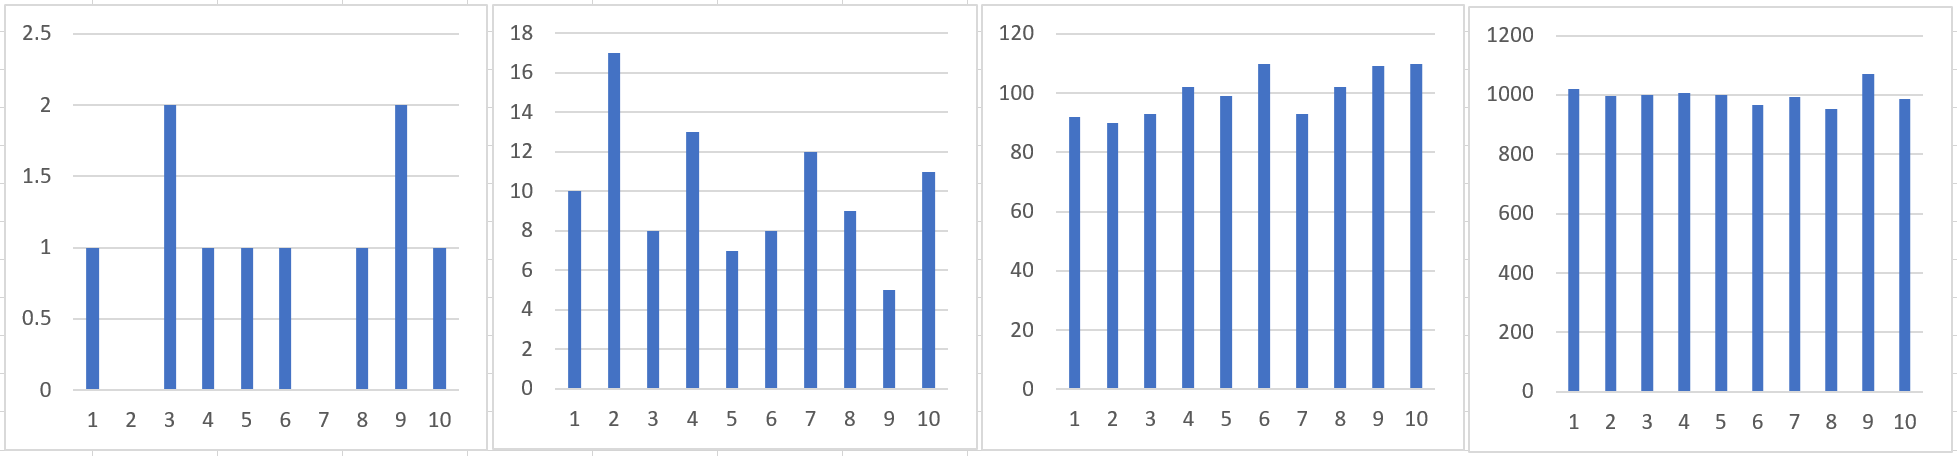
\includegraphics[width=\textwidth]{fig/2_histogram_uniform.png}
	\caption{Generating 10, 100, 1000, and 10000 values from $U\{1,10\}$ \label{fig:2_histogram_uniform}}
\end{figure}


\newpage

\section{The Bernoulli and Binomial Distributions}\label{sec2:binomial}

One of the most basic distributions is the \textbf{Bernoulli distribution}, where there are only two possibilities: \emph{success} or \emph{failure}, with a parameter $p$ describing probability of success, and a corresponding probability of $q = 1-p$ for failure.
Because there are only two possible outcomes, this is a discrete distribution.
Note that for $p = 0.5$ this is the discrete uniform distribution $U\{0,1\}$, and simulates a fair coin flip; for other values of $p$ it simulates an unfair coin flip.
We denote a Bernoulli-distributed random variable with parameter $p$ as $B(p)$.

The pdf of $B(p)$ is \[ f(k) = \left\{ \begin{matrix} 1-p, & k = 0 \cr p, & k = 1 \cr 0, & \text{ otherwise} \end{matrix} \right. \]
while its cdf is \[ g(k) = \left\{ \begin{matrix} 0, & k < 0 \cr 1-p, & 0 \leq k < 1 \cr 1, & k \geq 1 \end{matrix} \right. \]

\begin{figure}[htbp]
 \begin{minipage}{.5\textwidth}
        \centering
	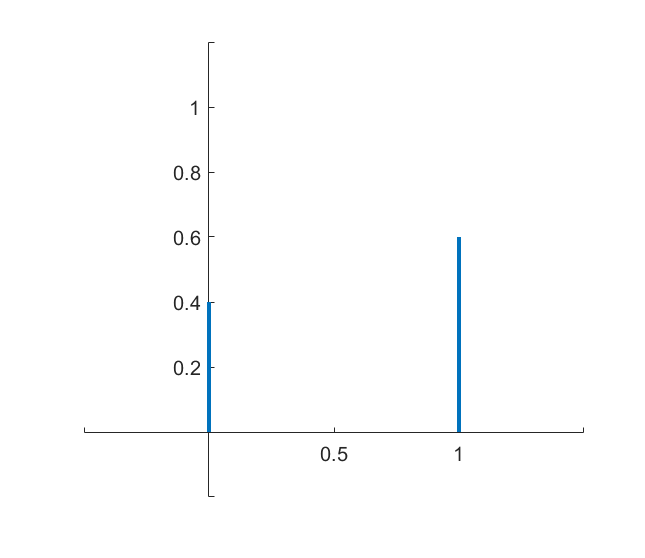
\includegraphics[width=0.9\linewidth]{fig/2_bernoulli_pdf}
    \end{minipage}
    \begin{minipage}{0.5\textwidth}
        \centering
	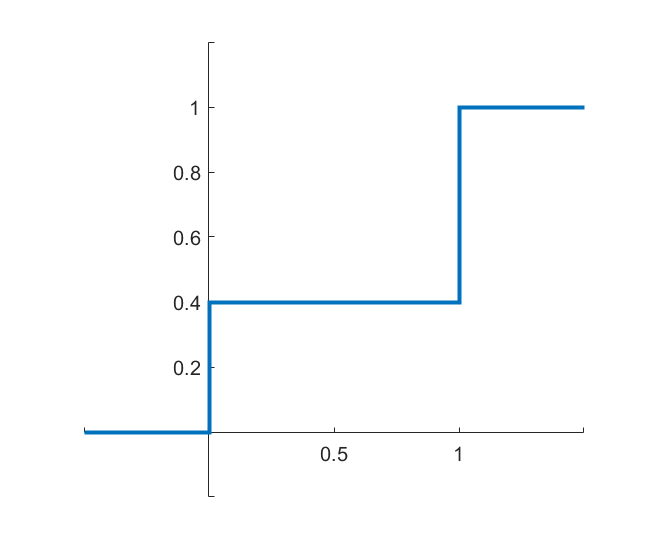
\includegraphics[width=0.9\linewidth]{fig/2_bernoulli_cdf}
    \end{minipage}	
    \caption{The pdf (L) and cdf (R) of the Bernoulli distribution with $p = 0.6$\label{fig:2_bernoulli_pdf}}
\end{figure}

To simulate this in Excel we use \texttt{RAND()} as well.
If $u$ was the result of \texttt{RAND()}, then we output $$\left\{\mat{\text{success,} & \text{if } 0 \leq u < p \cr \text{failure,} & \text{if } p \leq u < 1}\right. .$$

If we perform a Bernoulli trial multiple times, we get another distribution -- the \textbf{binomial distribution}, which counts the number of successes in $n$ independent Bernoulli trials.
Hence a binomially-distributed variable has two parameters - $p$ the probability of success for each trial, and $n$ the number of trials.
We denote this by $B(n,p)$ (so the Bernoulli distribution can also be written as $B(1,p)$).\footnote{So if $X_1, X_2, \ldots, X_n \sim B(1,p)$ independently, then $X_1 + X_2 + \cdots + X_n \sim B(n,p)$.}

\begin{myexample}
Consider the experiment of flipping two fair coins and counting the number of heads that come up.
This is a binomial random variable, with parameters $n = 2$ and $p = 0.5$.
There are three possible outcomes - zero, one, or two heads.
We can compute the probability of each outcome happening:

Ways to get zero heads: TT.

Ways to get one heads: HT or TH.

Ways to get two heads: HH.

Thus, we get the probabilities $\frac{1}{4},\frac{1}{2},\frac{1}{4}$ for each possible outcome. \qed
\end{myexample}

\begin{figure}[htbp]
 \begin{minipage}{.5\textwidth}
        \centering
	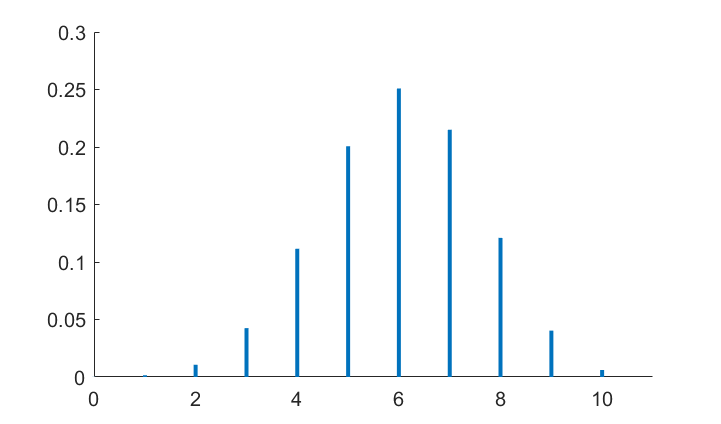
\includegraphics[width=0.9\linewidth]{fig/2_binomial_pdf}
    \end{minipage}
    \begin{minipage}{0.5\textwidth}
        \centering
	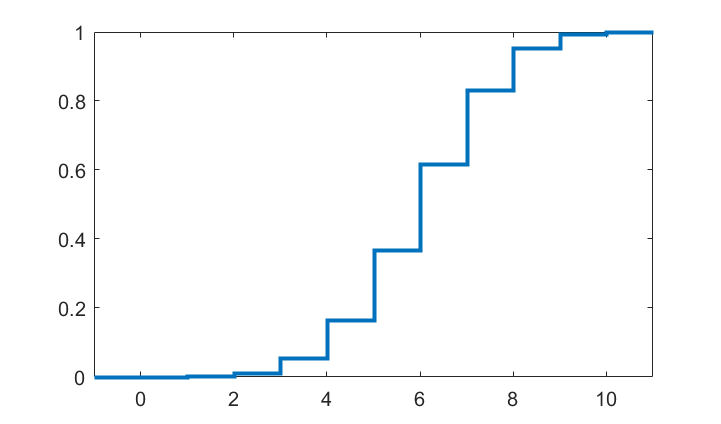
\includegraphics[width=0.9\linewidth]{fig/2_binomial_cdf}
    \end{minipage}	
    \caption{The pdf (L) and cdf (R) of the binomial distribution with $n = 10$ and $p = 0.6$\label{fig:2_binomial_pdf}}
\end{figure}



In Excel, multiple Bernoulli trials in separate cells can be used to simulate a binomial random variable by counting the number of successes.
Note in Figure~\ref{fig:excel_binomial} the use of the \texttt{IF} function -- it will output either 1 or 0 depending on whether the first condition \texttt{A3 < \$C\$1} is true or false.


\begin{figure}[htbp]
	\centering
	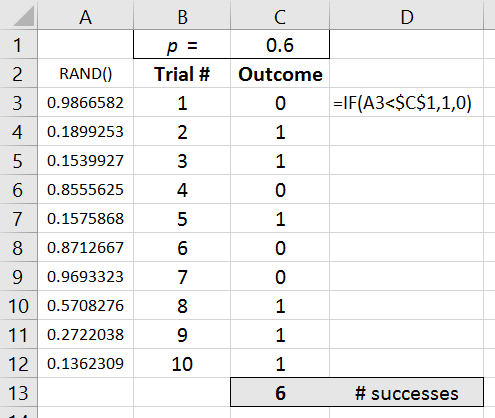
\includegraphics[width=0.35\textwidth]{fig/2_excel_binomial.png}
	\caption{Simulating multiple Bernoulli trials in Excel}
	\label{fig:excel_binomial}
\end{figure}

The exact probabilities of each outcome can be calculated analytically, and in Excel using the built-in \texttt{BINOM.DIST($x$,$n$,$p$,cumulative)}. 
This outputs the value of the pdf of $B(n,p)$ at $x$ when the argument \texttt{cumulative} is set to False. 
If \texttt{cumulative} is set to True, this function instead evaluates the cdf of $B(n,p)$ at $x$, or the probability of getting at most $x$ successes.

The function \texttt{BINOM.INV($n$,$p$,prob)} computes the inverse of \texttt{BINOM.DIST}, and can be used to generate samples from the binomial distribution.
It outputs, given the parameters $n$, $p$, and a given probability \texttt{prob}, the smallest integer for which the cumulative binomial distribution is at least \texttt{prob}.
Hence we can generate binomially-distributed variates by using \texttt{RAND()} as an input.
Figure~\ref{fig:2_excel_binominv} illustrates this process while Figure~\ref{fig:2_binomial_cdf_inv} shows the inverse of the cdf for $B(10,0.6)$.

\begin{figure}[htbp]
\centering
 \begin{minipage}{.45\textwidth}
        \centering
	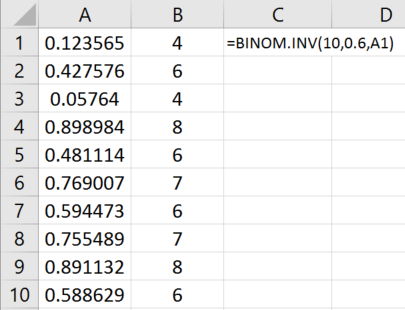
\includegraphics[width=0.9\textwidth]{fig/2_excel_binominv2.png}
	\captionsetup{font=small}
	\caption{10 outcomes from $B(10,0.6)$ \label{fig:2_excel_binominv}}
    \end{minipage}
    \begin{minipage}{0.55\textwidth}
        \centering
	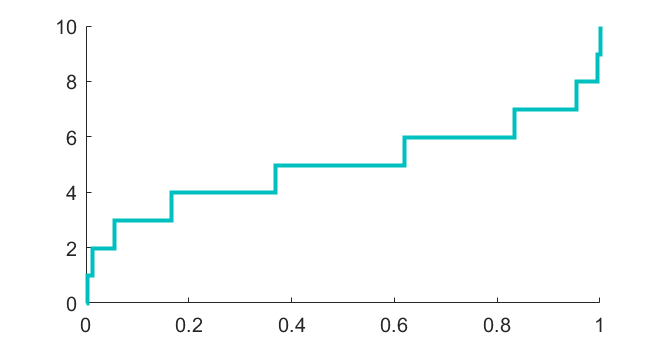
\includegraphics[width=0.95\textwidth]{fig/2_binomial_cdf_inv.png}
	\captionsetup{font=small}
	\caption{The inverse of the cdf for $B(10,0.6)$ \label{fig:2_binomial_cdf_inv}}
    \end{minipage}	
\end{figure}


In Figure~\ref{fig:2_histogram_binomial} we show the result of using Excel to generate 10, 100 and 1000 outcomes from $B(10,0.6)$.
Observe that outcomes are clustered around $6$ and that the curve has a distinct `bell' shape.
We discuss this phenomenon in Section~\ref{sec2:normal}.


\begin{figure}[htbp]
	\centering
	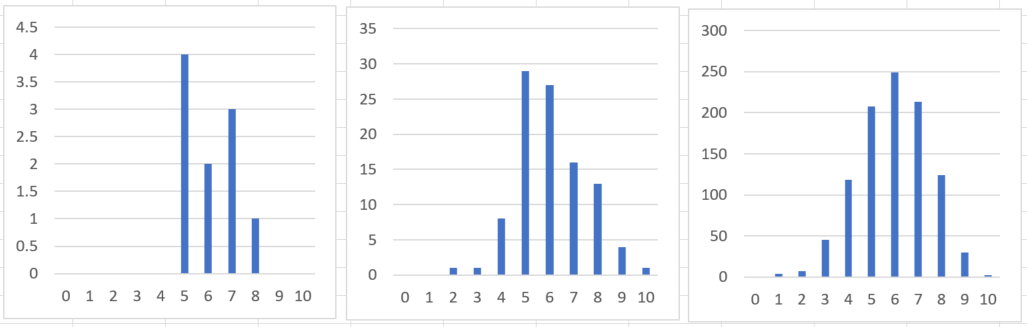
\includegraphics[width=0.75\textwidth]{fig/2_histogram_binomial.png}
	\caption{Generating 10, 100, and 1000 outcomes from $B(10,0.6)$ in Excel \label{fig:2_histogram_binomial}}
\end{figure}




\section{The Continuous Uniform Distribution, PDFs and CDFs}

We discussed in Section~\ref{sec2:discreteuni} the discrete uniform distribution $U\{a,b\}$, where each outcome in the set $\{a,a+1,a+2,\ldots,b\}$ is equally likely.

There is also a continuous version of this distribution, where the possible set of outcomes is an interval of real numbers.
Let us denote by $U(a,b)$ the continuous uniform distribution on the interval $[a,b]$.
Sampling a value $u$ from the standard continuous uniform distribution $U(0,1)$ is exactly what the \texttt{RAND()} function in Excel is designed to approximate.\footnote{Note that since the sample space is an infinite set, the probability of generating any specific value from $U(0,1)$ is 0.}
We can use $u$ to simulate the random variable $U(a,b)$, using the transformation $a + (b-a)u.$

\textbf{Question}: Do continuous random variables have probability density functions?

The answer to this question is \emph{yes}, but we will have to define them differently.
Since continuous random variables have infinitely many possible outcomes, we do not want to talk about probabilities of individual outcomes, but instead, the probability that an outcome will lie \emph{in a given interval}.

To illustrate, suppose we know that $X \sim U(0,2)$.
Then, intuitively, the probability that $X < 0.5$ should be $0.25$, which is the length of the interval $[0,0.5)$ divided by the length of the interval $[0,2)$.

So, for a continuous random variable $X$, its \textbf{probability density function} or \textbf{pdf} is a function $f(x)$, that satisfies the property that 
\begin{center}$P(a \leq X \leq b) = $ the area under the graph of $f(x)$ in between $x = a$ and $x = b$. \footnote{If you have taken integral calculus you may recognize this as the integral of $f(x)$ from $a$ to $b$: \\ $ P(a \leq x \leq b) = \int_a^b f(x) \, dx .$}\end{center}

\vspace{-0.3cm}
For example, for $U(a,b)$, its pdf is $f(x) = \left\{ \begin{matrix} \frac{1}{b-a}, & a \leq x \leq b \cr 0, & \text{ otherwise}\end{matrix} \right.$.

The \textbf{cdf} $g(x)$ of a continuous random variable is defined in the same way: \[ g(x) = P(X \leq x).\]
The cdf of $U(a,b)$ is \[ g(x) = \left\{ \begin{matrix} \frac{x-a}{b-a}, & a \leq x \leq b \cr 0, & \text{ otherwise} \end{matrix} \right. . \]

For now, do not worry about dealing with these functions themselves; what is more important is that we know how to simulate these random variables using Excel.

\begin{figure}[htbp]
 \begin{minipage}{.5\textwidth}
        \centering
	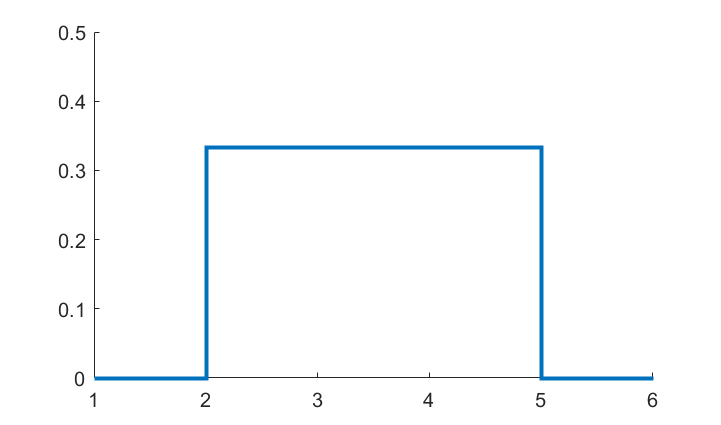
\includegraphics[width=0.9\linewidth]{fig/2_uni_pdf}
    \end{minipage}
    \begin{minipage}{0.5\textwidth}
        \centering
	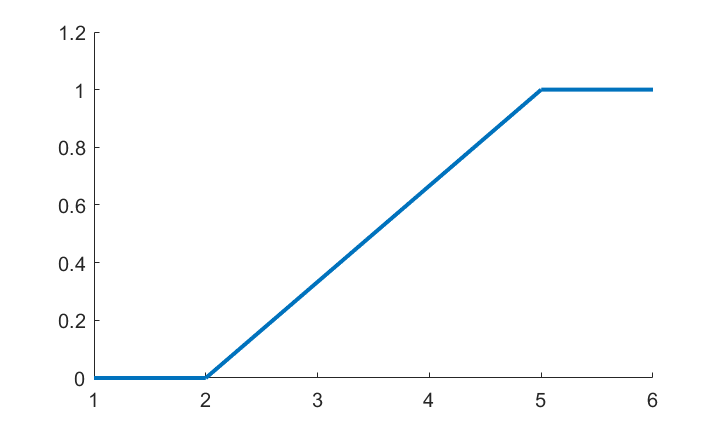
\includegraphics[width=0.9\linewidth]{fig/2_uni_cdf}
    \end{minipage}	
    \caption{The pdf (L) and cdf (R) of the continuous uniform distribution $U(2,5)$\label{fig:2_uni_pdf}}
\end{figure}

\subsection{Application: Area and Volume Computations}\label{sec2:areavolume}

One surprising application of the continuous uniform distribution is the approximation of quantities that are not random at all: areas, volumes, and their higher-dimensional analogues.
For instance, suppose we want to calculate the area of the quarter-circle in Figure~\ref{fig:4_quartercircle}.

\begin{wrapfigure}{r}{5.5cm}
	\centering
	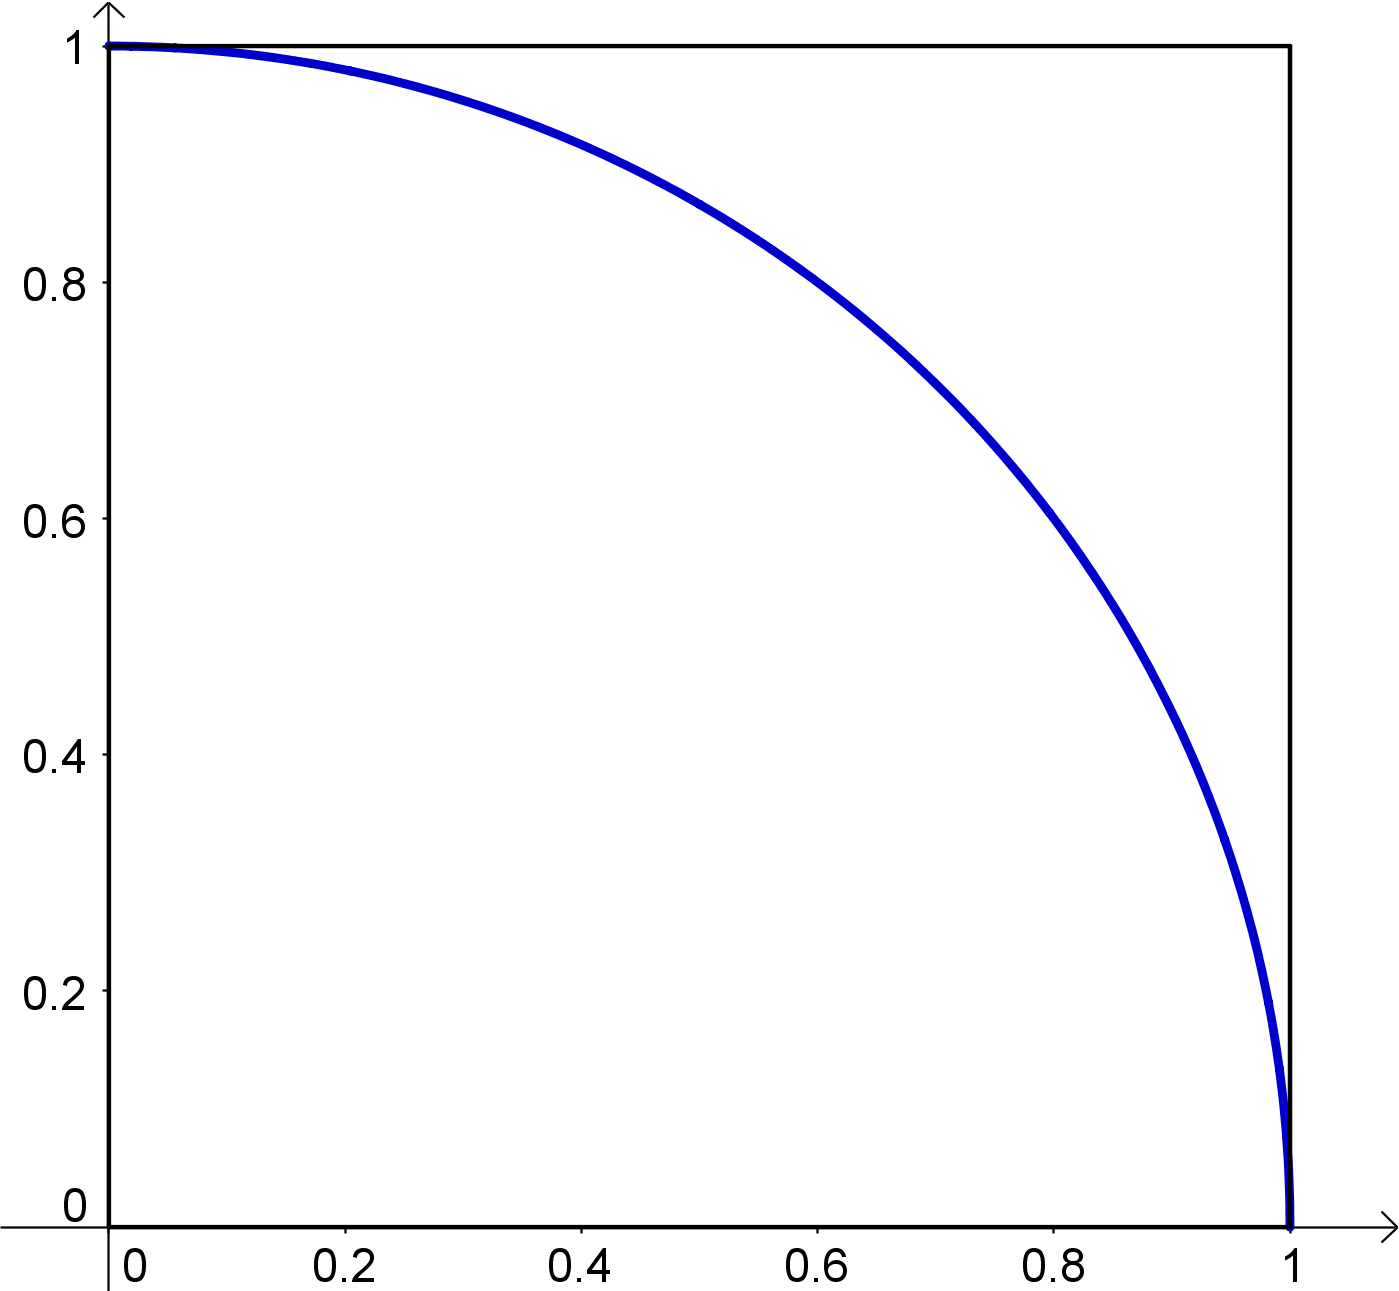
\includegraphics[width=4.8cm]{fig/4_quartercircle.png}
	\caption{\label{fig:4_quartercircle}}
\end{wrapfigure}

We know from grade-school geometry that this area is equal to $\frac{\pi}{4}$.
We can also approximate this area as follows.
We generate points at random inside the unit square, count the number of points inside the given region, and divide this by the total number of points generated.
Since the unit square has area 1, the result will be an approximation of the area of the given region.

\iffalse

\begin{figure}[htbp]
	\centering
	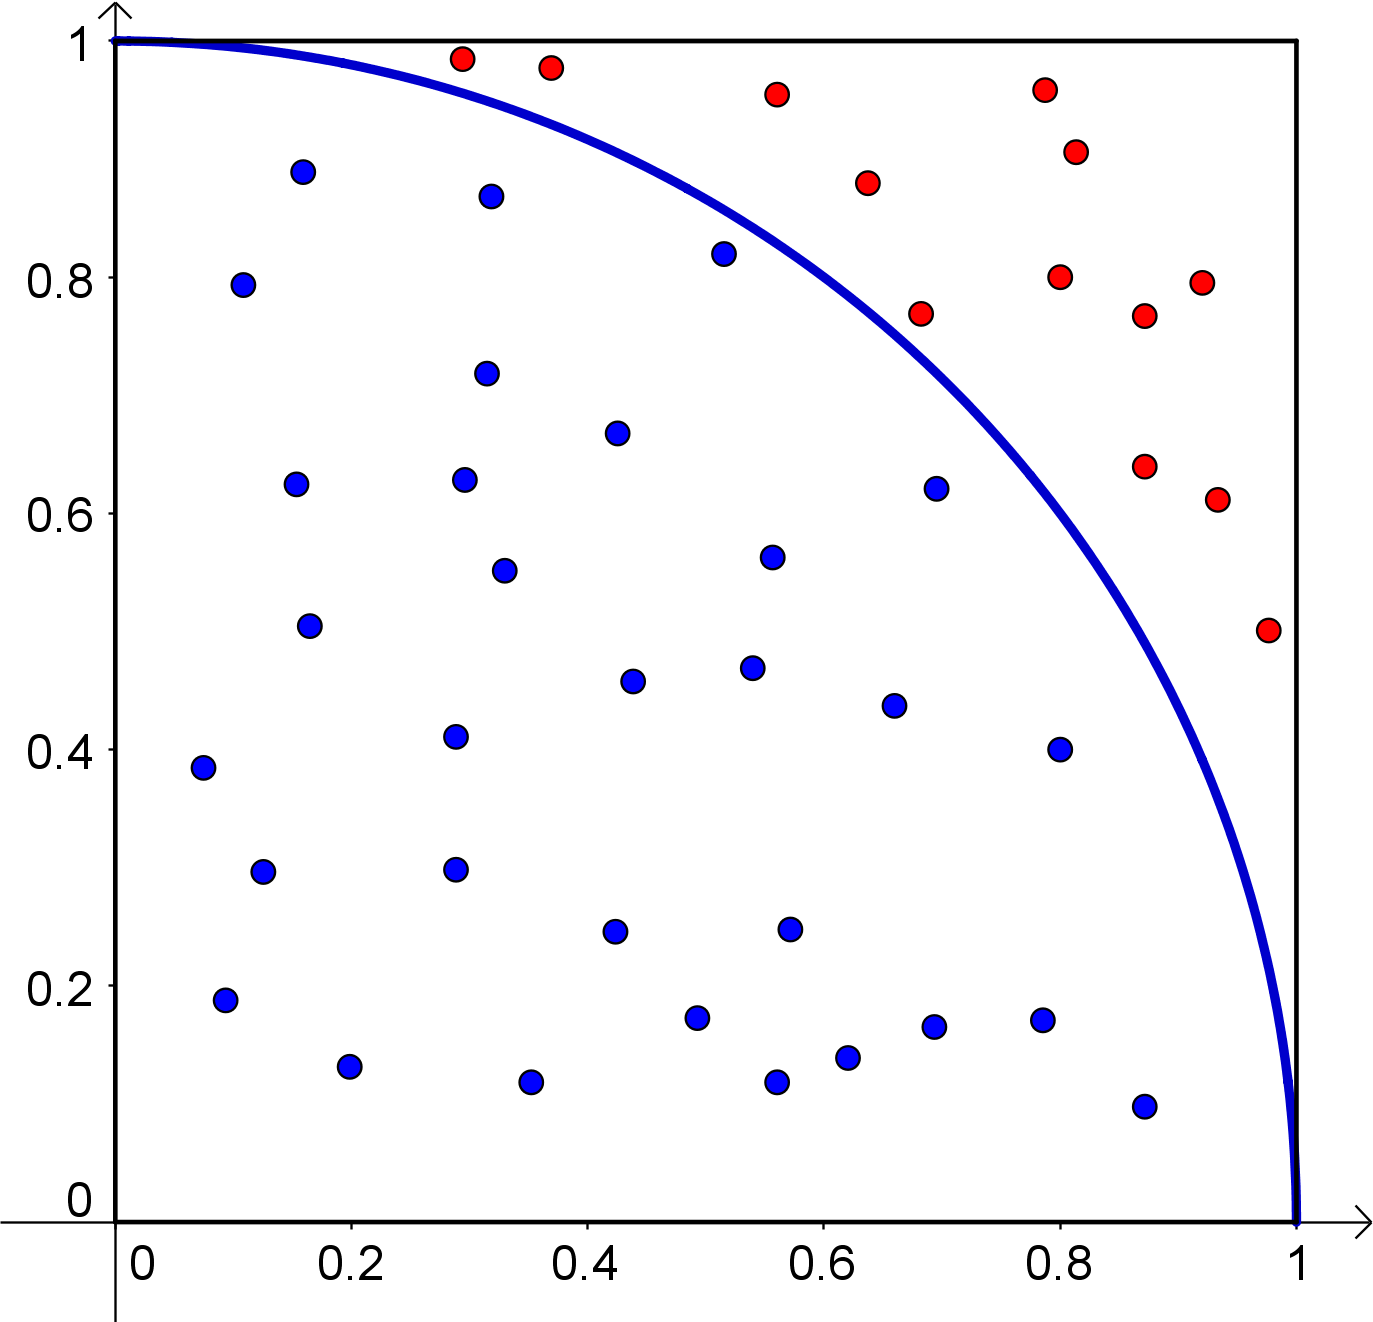
\includegraphics[width=0.4\textwidth]{fig/4_quartercircle_points.png}
	\caption{The area of the region is roughly the number of blue points divided by the total number of points generated. \label{fig:4_quartercircle_points}}
\end{figure}
\fi

This is easy to do.
Since the area under consideration is contained within the unit square $[0,1] \times [0,1]$, we can uniformly pick a point inside the square at random by using \texttt{RAND()} for each coordinate.
It is also simple to check whether a point is inside this circle: test if its distance from the origin is less than 1.
The following figures show the results of generating 20, 200, and 2000 points in this manner.

\begin{figure}[htbp]
    \begin{minipage}{0.3\textwidth}
        \centering
	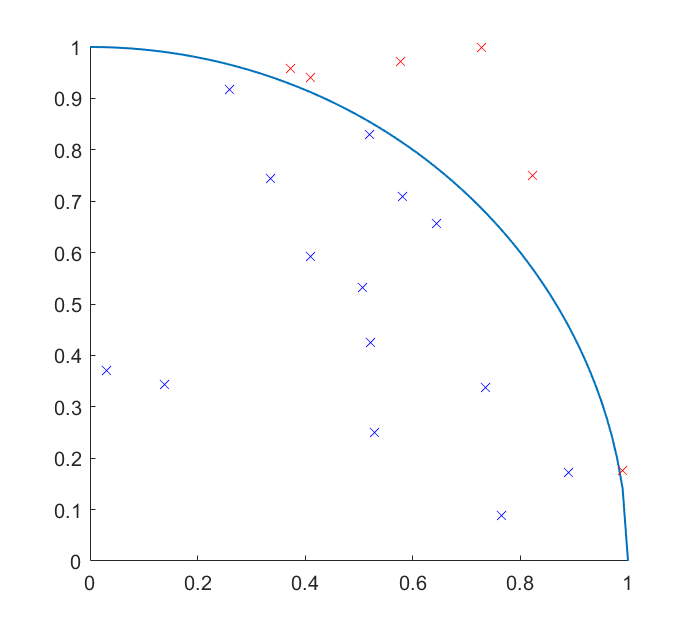
\includegraphics[width=\linewidth]{fig/4_quartercircle_1plot.png}
    \end{minipage}
    \hfill
    \begin{minipage}{0.3\textwidth}
        \centering
	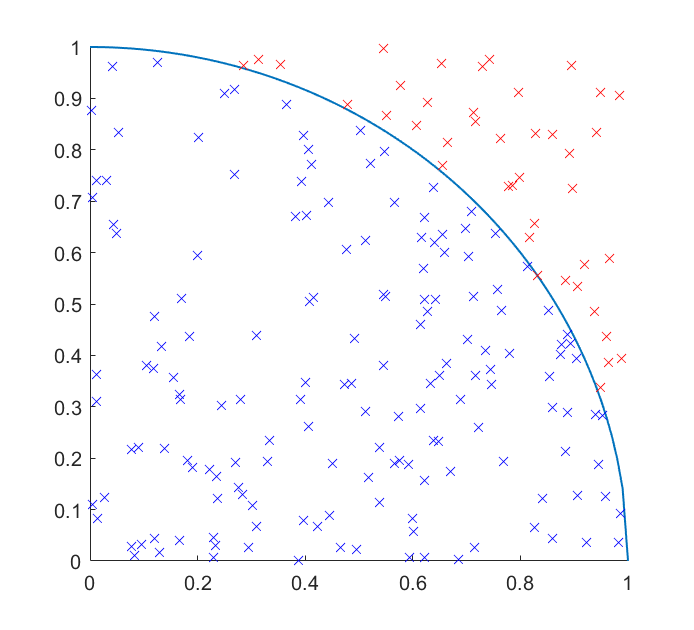
\includegraphics[width=\linewidth]{fig/4_quartercircle_2plot.png}
    \end{minipage}
    \hfill
    \begin{minipage}{0.3\textwidth}
        \centering
	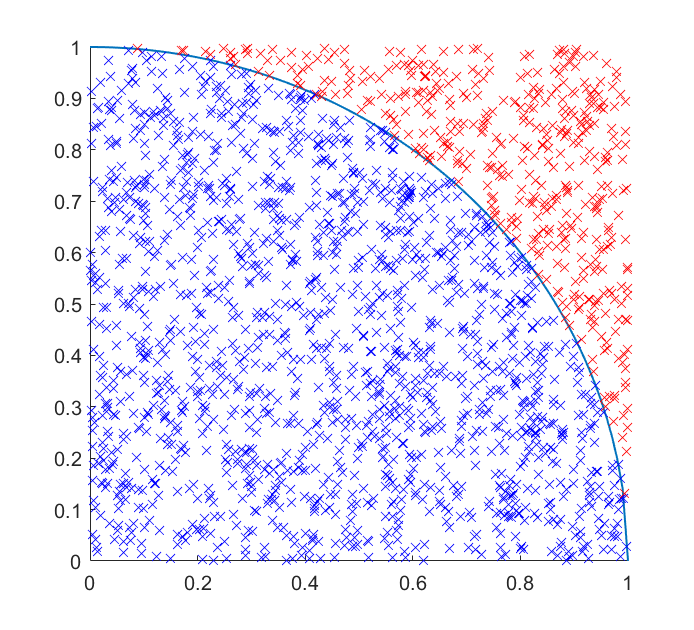
\includegraphics[width=\linewidth]{fig/4_quartercircle_3plot.png}
    \end{minipage}	
    \caption{20, 200, and 2000 randomly-generated points. \label{fig:4_quartercircleplots}}
\end{figure}

\newpage

\begin{figure}[htbp]
	\centering
	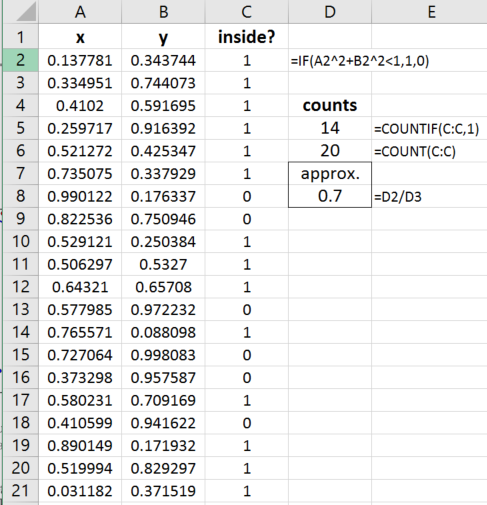
\includegraphics[width=0.5\textwidth]{fig/4_quartercircle_1.png}
	\caption{Area approximation of the quarter circle using 20 random points. \label{fig:4_quartercircle_1}}
\end{figure}

\begin{figure}[htbp]
    \begin{minipage}{0.45\textwidth}
        \centering
	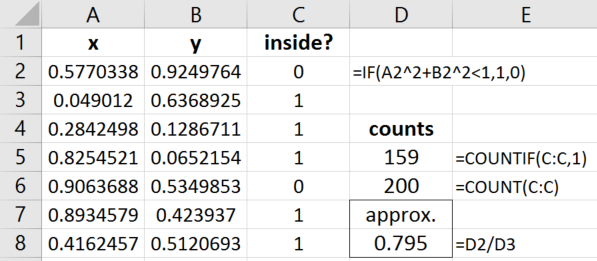
\includegraphics[width=\linewidth]{fig/4_quartercircle_2.png}
    \end{minipage}
    \hfill
    \begin{minipage}{0.45\textwidth}
        \centering
	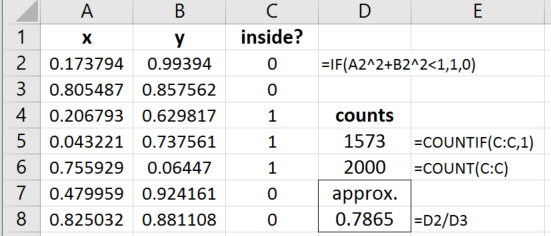
\includegraphics[width=\linewidth]{fig/4_quartercircle_3.png}
    \end{minipage}	
    \caption{Area approximations using 200 and 2000 random points. \label{fig:4_quartercircle_23}}
\end{figure}


A big advantage of this method is that it can be easily implemented when we have a way to test if a point in the set.
This is the case, for instance, if the set is the area under a curve.


Another approach to an area calculation like this involves breaking up the space $[0,1]\times[0,1]$ around the region into smaller squares, and colouring the squares whose centre is in the region under consideration -- see Figure~\ref{fig:4_heart} for an example.
Summing the areas of the coloured squares gives an estimate of the area; taking the limit of this as the squares get smaller is effectively equivalent to the integration technique from calculus.


\begin{figure}
\centering
    \begin{minipage}{0.3\textwidth}
        \centering
	
\includegraphics[width=0.85\linewidth]{fig/4_heart.png}
    \end{minipage}%
    \begin{minipage}{0.3\textwidth}
        \centering
	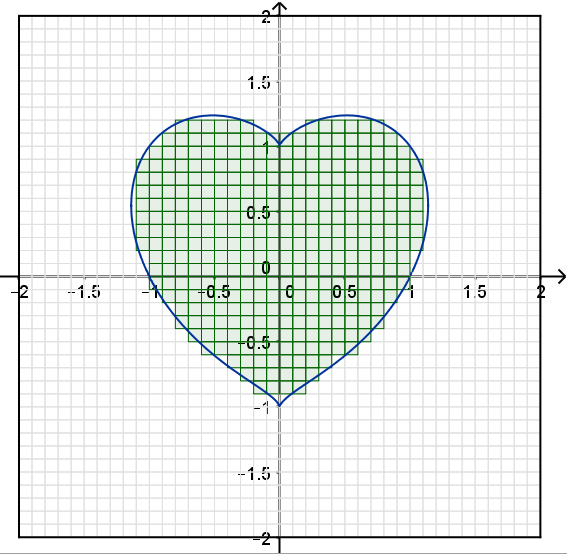
\includegraphics[width=0.85\linewidth]{fig/4_heart_sq.png}
    \end{minipage}	
    \caption{Approximating the area of a general region. \label{fig:4_heart}}
\end{figure}



But there are situations when one would prefer a random process (dropping points randomly and calculating the proportion) over a deterministic one (computing the integral, or estimating it from a count of grid points).
For instance, in two dimensions using an evenly-spaced grid makes sense, while in twenty-dimensional space it may not.
In particular, in high dimensions, grids have too many points: in dimension 20 the unit cube has over a million vertices and a $3 \times 3 \times \cdots \times 3$ grid has more than three trillion points while missing huge spaces inside the cube.
It is very difficult to find a deterministic way of producing well-spaced points in high dimension.
The method of using random points to estimate areas is called \emph{Monte Carlo integration}.


\section{The Normal Distribution, more PDFs and CDFs}\label{sec2:normal}

The \textbf{normal distribution} is often called the \textbf{Gaussian distribution} or the \textbf{bell curve}.
The two parameters associated with this distribution are the \emph{mean} $\mu$ and the \emph{standard deviation} $\sigma$.
Random variables drawn from this distribution will tend to be gathered around the mean, while the variance measures how `spread out' values are (a lower variance means values are more likely to stay close to the mean).
This distribution is denoted as $N(\mu, \sigma)$, and is one of the most important statistical distributions, because it is commonly seen in nature. For instance, in error analysis, measurement errors are modelled by the normal distribution (e.g. when calibrating instruments, etc).

In Figure~\ref{fig:2_normal} we show the probability density function of the standard normal distribution $N(0,1)$.
The density function for $N(\mu,\sigma)$ is 
$$f(x) = \frac{1}{\sigma\sqrt{2\pi}}e^{-\frac{1}{2}\left(\frac{x-\mu}{\sigma}\right)^2}.$$

\begin{figure}[htbp]
	\centering
	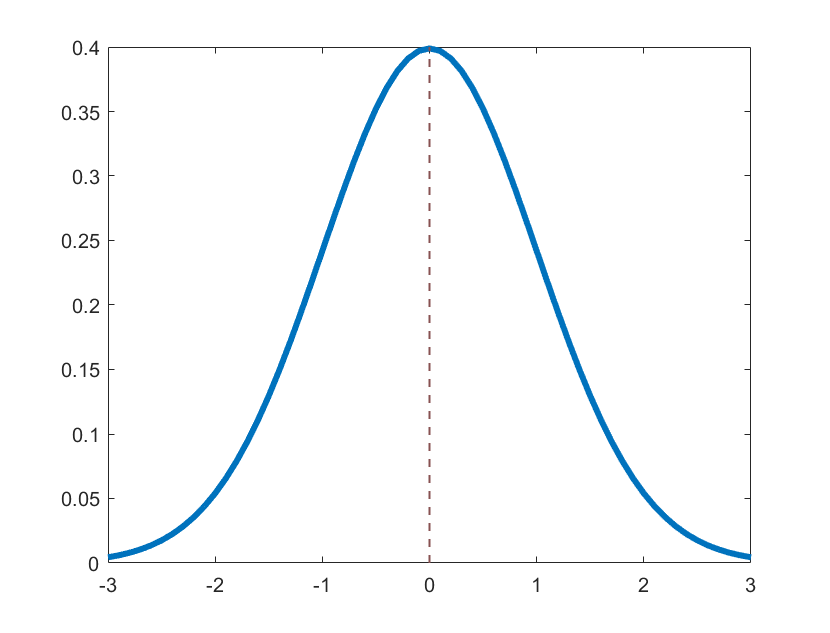
\includegraphics[width=0.5\textwidth]{fig/2_normal.png}
	\caption{The probability density function of the normal distribution $N(0,1)$ \label{fig:2_normal}}
\end{figure}

In Excel, the cumulative probability $P(Z < k)$ for $Z \sim N(\mu,\sigma)$ is calculated by the function \texttt{NORM.DIST(k,$\mu$,$\sigma$,cumulative)} function when the parameter \texttt{cumulative} is set to True (if it is set to False, it just outputs the value of the probability density function at that $k$). 
The function \texttt{NORMINV(prob,$\mu$,$\sigma$)} is the inverse of this; it calculates the point $k$ for which $P(Z < k) = $ \texttt{prob}.

\begin{figure}[htbp]
 \begin{minipage}{.5\textwidth}
        \centering
	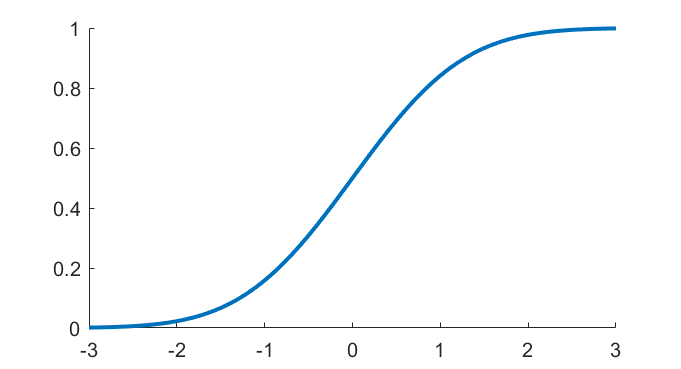
\includegraphics[width=0.9\linewidth]{fig/2_normal_cdf}
    \end{minipage}
    \begin{minipage}{0.5\textwidth}
        \centering
	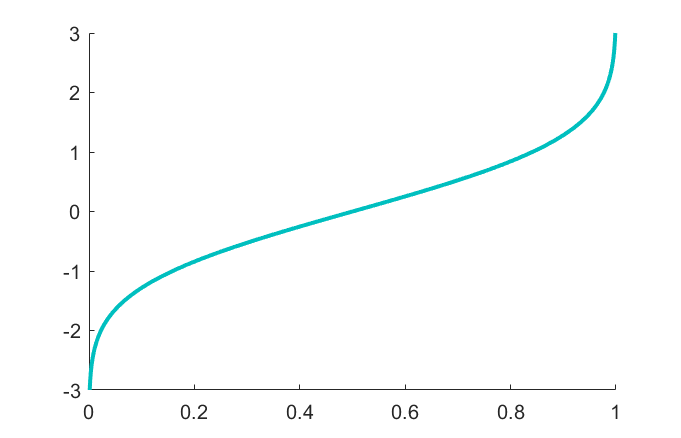
\includegraphics[width=0.9\linewidth]{fig/2_normal_cdf_inv}
    \end{minipage}	
    \caption{The cdf (L) and its inverse (R) for the standard normal distribution $N(0,1)$\label{fig:2_normal_cdf}}
\end{figure}

\begin{myexample}\label{ex:2_normal_example}
Suppose that we sample from a normal distribution with mean $\mu = 50$ and standard deviation $\sigma = 10$. What is the probability that the random sample is (a) smaller than 40? (b) in between 60 and 70?

\underline{Solution}
Using \texttt{NORM.DIST} in Excel, we can compute the required probabilities.
For (a), we get \texttt{NORM.DIST(40,50,10,TRUE)} $ = 0.158655$.
This is also equal to the area under the curve of $N(50,10)$ from $x = 0$ to $40$.

(b) This is calculated by the formula $$\texttt{NORM.DIST(70,50,10,TRUE)-NORM.DIST(60,50,10,TRUE)} = 0.135905,$$ and this is the area under the curve of $N(50,10)$ from $x = 60$ to $x = 70$. \qed
\end{myexample}

\begin{figure}[htbp]
 \begin{minipage}{.5\textwidth}
        \centering
	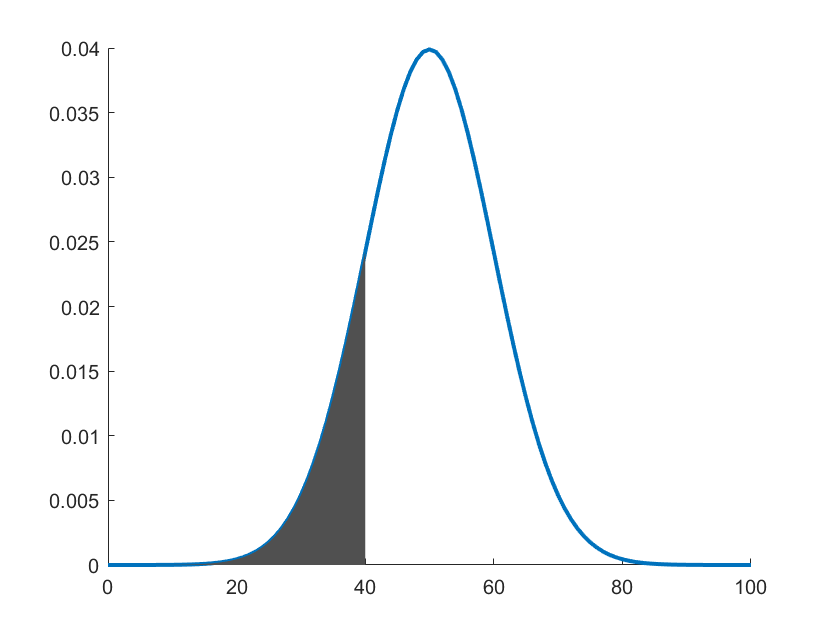
\includegraphics[width=0.9\linewidth]{fig/2_normal_example_a}
    \end{minipage}
    \begin{minipage}{0.5\textwidth}
        \centering
	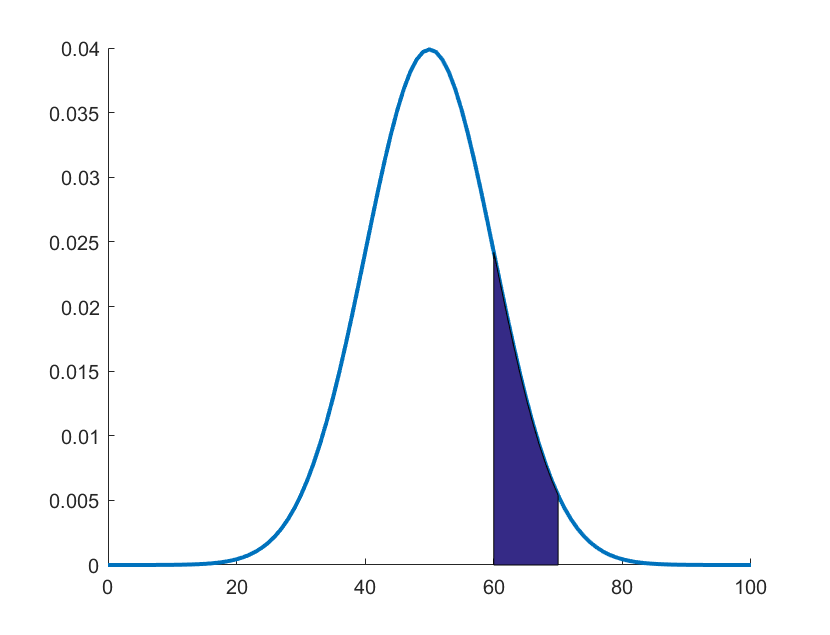
\includegraphics[width=0.9\linewidth]{fig/2_normal_example_b}
    \end{minipage}	
    \caption{The probabilities in Example~\ref{ex:2_normal_example} as areas under the normal curve \label{fig:2_normal_example}}
\end{figure}

To generate values from a normal distribution in Excel, one could just call the \texttt{NORMINV()} function with a random probability for its first argument.
For instance, the formula \texttt{NORMINV(RAND(),50,10)} will generate values from $N(50,10)$, as is illustrated in Figure~\ref{fig:2_normal_excel}.

\begin{figure}[htbp]
	\centering
	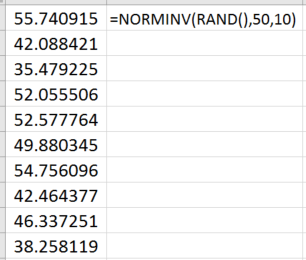
\includegraphics[width=0.3\textwidth]{fig/2_normal_excel.png}
	\caption{Generating values from $N(50,10)$ \label{fig:2_normal_excel}}
\end{figure}

\begin{myexample}
The heights of women in a certain country are normally-distributed with mean $\mu = 65$in and standard deviation $\sigma = 5$in. What is the probability that a randomly-selected person from this country is taller than 6ft?

\underline{Solution}: The probability is \texttt{1 - NORM.DIST(72,65,5,TRUE)} $ = .008076$, or 0.81\%. \qed
\end{myexample}

\section{The Exponential Distribution}\label{sec:2_expo}

The \textbf{exponential distribution} is another widely-used distribution in applications, since it models interarrival times between two events -- for example, the time it takes between customers at the bank, or the amount of time in between calls at a customer service centre.
It also models the lifetimes of electrical equipment.
This distribution is denoted as Exp$(\lambda)$, with the single parameter $\lambda > 0$ representing the average rate of arrivals/services per unit time.
The probability density function for Exp$(\lambda)$ is the following: 
\[f(x) = \left\{ \begin{matrix} \lambda e^{-\lambda x}, & x \geq 0 \cr 0, & \text{elsewhere} \end{matrix} \right. \]

\vspace{-0.5cm}

\begin{figure}[htbp]
	\centering
	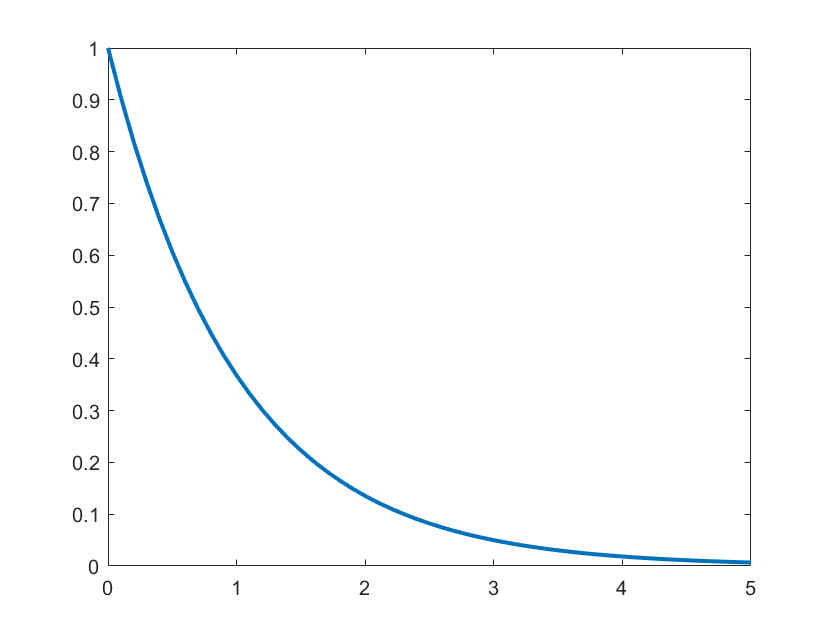
\includegraphics[width=0.5\textwidth]{fig/2_expo.png}
	\caption{The probability density function of the exponential distribution Exp$(1)$ \label{fig:2_expo}}
\end{figure}

As this is a continuous distribution, we will use cumulative probabilities $P(X < k)$ to describe events.
If $X \sim $ Exp$(\lambda)$, then its cdf is \[ P(X < k) = 1 - e^{-\lambda k}, k \geq 0.\]

\begin{myexample}\label{2:expo_example}
Suppose that 10 customers arrive at a restaurant per hour on average.
Find the probability that when the restaurant opens, the first customer arrives in the first 6 minutes.

\underline{Solution}: The interarrival times of customers is an exponentially-distributed random variable with $\lambda = 10$, or $X \sim \text{Exp}(10)$. Hence $P(X < 0.1) = 1 - e^{-10(0.1)} = 0.632121$, or 63.21\%. \qed
\end{myexample}

\begin{figure}[htbp]
	\centering
	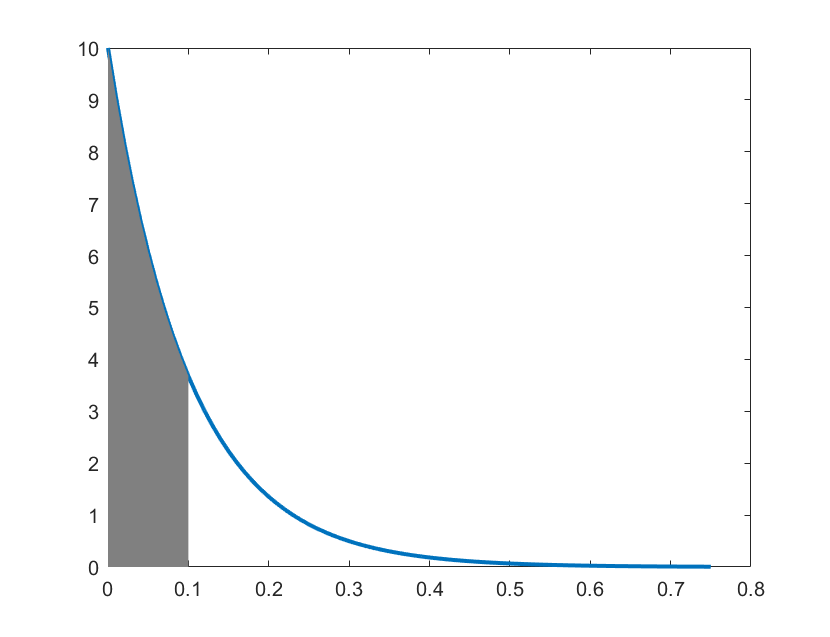
\includegraphics[width=0.5\textwidth]{fig/2_expo_example.png}
	\caption{The probability density function for Exp$(10)$ and the probability $P(X < 0.1)$. \label{fig:2_expo_example}}
\end{figure}


To calculate the cumulative probability $P(X < k)$ in Excel, the function is \\ \texttt{EXPON.DIST(k,lambda,TRUE)}, with the last parameter again indicating either the pdf (False) or the cdf (True).
However there is no built-in function for its inverse as in the normal distribution, since it has a simple algebraic expression: if $P(X < k) = y = 1 - e^{-\lambda k}$, then $k = -\frac{\ln(1-y)}{\lambda}$.
Hence we can randomly generate exponentially-distributed variables by using $y = $ \texttt{RAND()}, then computing $k$ from this expression.

\begin{figure}[htbp]
	\centering
	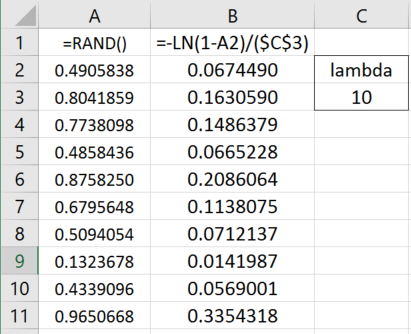
\includegraphics[width=0.4\textwidth]{fig/2_expo_excel.png}
	\caption{Ten values generated from Exp$(10)$ using \texttt{RAND()} and the inverse cumulative distribution function \label{fig:2_expo_excel}}
\end{figure}

One important property of the exponential function is that it is \emph{memoryless}, in that it models the time in between two events \emph{regardless of how many times that event has happened}.
In Example~\ref{2:expo_example}, this means that after the first customer has arrived, the time it takes for the second customer to arrive is also modelled by Exp($10$).
Similarly for the third, fourth, etc.
This is a common assumption when modelling queueing processes.

\iffalse

\section{The Poisson Distribution}

The \textbf{Poisson distribution} is a discrete distribution that is closely related to the exponential distribution.
For a Poisson-distributed random variable $X$ with parameter $\mu$, it has a \emph{probability density function} given by $$p(k) = P(X = k) = \left\{ \begin{matrix} \dfrac{e^{-\mu}\mu^k}{k!}, & k = 0,1,2,\ldots \cr \cr 0, & \text{ otherwise}\end{matrix} \right.$$
While the exponential distribution models waiting time in between two events, the Poisson distribution models the number of events that occur in a fixed time interval.
In fact, using this property we can use the exponential distribution to generate samples from the Poisson distribution:

Let $X \sim $ Pois$(\mu)$, and suppose $X_1, X_2, X_3, \ldots \sim $ Exp$(\mu)$.
Then $X = k$ if and only if \[ X_1 + X_2 + \cdots + X_k \leq 1 < X_1 + X_2 + \cdots + X_k + X_{k+1} \]

What this means is that to randomly generate from Pois$(\mu)$, we can generate values from Exp$(\mu)$ until their sum becomes larger than 1.
Then the Poisson value is one less than the number of values generated -- see Figure~\ref{fig:2_poisson}.

\begin{figure}[htbp]
	\centering
	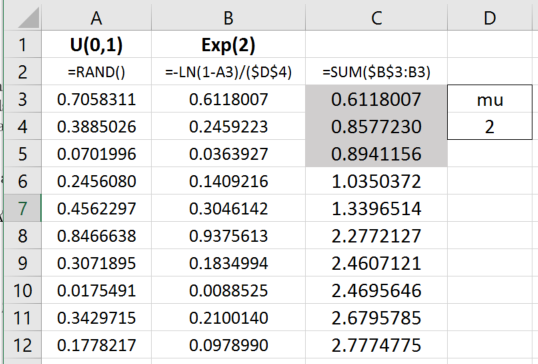
\includegraphics[width=0.5\textwidth]{fig/2_poisson.png}
	\caption{Generating a Poisson value randomly using the exponential distribution. Here the generated value is 3, since after 4 exponential values the sum becomes larger than 1. \label{fig:2_poisson}}
\end{figure}

This method is slightly more difficult to implement in Excel, especially for generating multiple Poisson values.
One would have to use some logical statements and checks (using the \texttt{IF()} function) to be able to do this multiple times.
In the next section we go over some features in Excel that allow us to generate multiple random variables.


\section{Data Tables}

To repeatedly generate random numbers in Excel, we use \textbf{data tables}.
These are used in Excel for scenario analysis -- recomputing a formula using different inputs.

\begin{myexample}
Suppose that for MATH208W your marks for each component are 30/40 for Assignments, 12/15 for the Midterm, and 20/20 for the Final Project.
Say you wanted to compute your final grade when your Final Exam mark is 5, 10, 15, 20, or 25/25.

First, input the individual components in Excel with a formula for the total, then create a column with the potential Final Exam marks you want to check.
In the column beside that, enter a formula referring to the output value you would like to track (\texttt{B5}).

\begin{figure}[htbp]
	\centering
	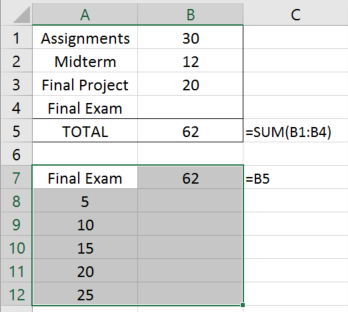
\includegraphics[width=0.5\textwidth]{fig/2_data_table_exA.png}
	\label{fig:2_data_table_exA}
\end{figure}

Next, highlight the two columns in the table you want to produce (in this example, \texttt{A7:B12}), then go to Data $\rightarrow$ What-If Analysis $\rightarrow$ Data Table.
For `column input cell' enter the cell whose value you would like to change.
Clicking Enter will generate the desired values.



\begin{figure}[htbp]
 \begin{minipage}{0.55\textwidth}
        \centering
	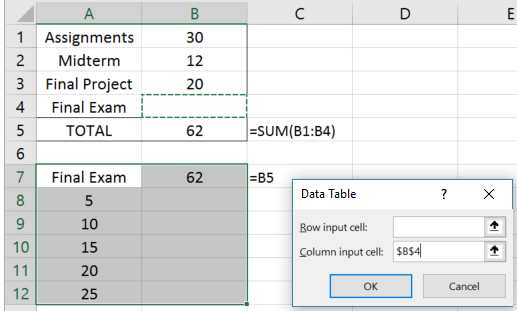
\includegraphics[width=\linewidth]{fig/2_data_table_exB.png}
    \end{minipage}
    \quad $\Rightarrow$ \quad
    \begin{minipage}{0.37\textwidth}
        \centering
	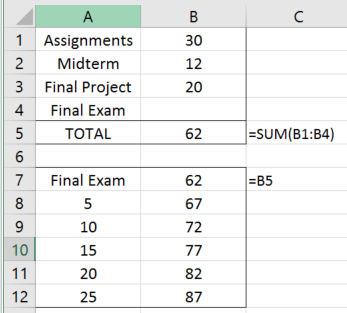
\includegraphics[width=\linewidth]{fig/2_data_table_exC.png}
    \end{minipage}	
    \caption{Using a data table in Excel. \label{fig:2_data_table_ex}}
\end{figure}

Note this is very basic; many real-world scenarios can be analyzed using this tool. \qed


\end{myexample}

Essentially, data tables do the work of entering information and recalculating the worksheet based on the changes.
For random number generation this is especially useful -- recall that each time the worksheet is refreshed/recomputed, each call to \texttt{RAND()} will refresh as well.

In Figure~\ref{fig:excel_binomial}, we generated a value from the binomial distribution $B(10,0.6)$.
By using a data table we can generate multiple values.
However since we are not changing any inputs (just refreshing the worksheet) the column input cell can be any empty cell.

\vspace{1cm}

\begin{figure}[htbp]
	\centering
	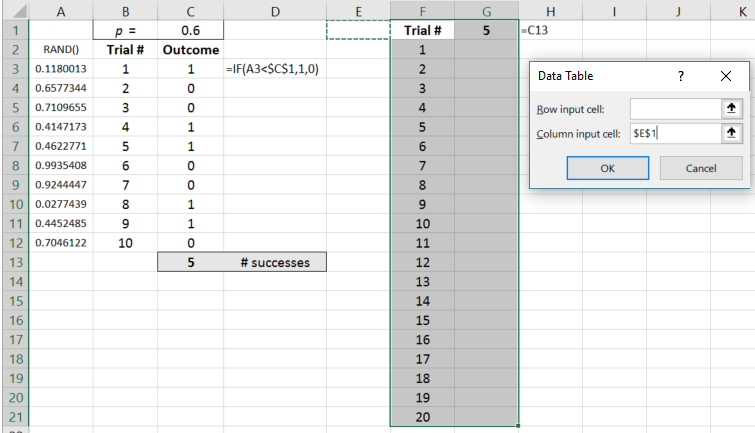
\includegraphics[width=0.9\textwidth]{fig/2_data_table_binomialA.png}
	\caption{Using a data table to generate binomial variates \label{fig:2_data_table_binomialA}}
\end{figure}

\begin{figure}[htbp]
	\centering
	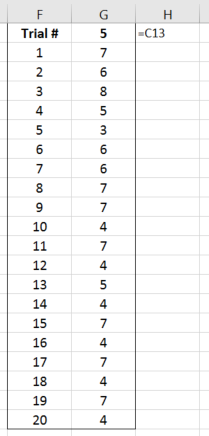
\includegraphics[width=0.3\textwidth]{fig/2_data_table_binomialB.png}
	\caption{Result of data table \label{fig:2_data_table_binomialB}}
\end{figure}

\fi

\newpage

\begin{center}
	\textbf{EXERCISES}
\end{center}

\begin{enumerate}[label={2.\arabic*},leftmargin=1cm]
	\item A pair of dice is rolled; let $X$ be the sum of the two numbers that appear. Tabulate the pdf for $X$. \label{2ex:pdf}
	\item Plot the cdf of the random variable $X$ of Exercise~\ref{2ex:pdf}
	\item \textbf{Explore}. We can simulate drawing a card at random from a standard deck of cards using $U\{1,52\}$, by assigning cards to numbers (1-13 are the A-K of clubs, 14-26 are diamonds, 27-39 hearts, and 40-52 spades).
		\begin{enumerate}[(a)]
			\item In Excel, generate 20 numbers from $U\{1,52\}$ and list the cards they correspond to. Do you see any repeats? How about when you generate 40 numbers?
			\item Guess the average number of draws from a deck of cards until \emph{the first repeat occurs}, assuming the draws are done with replacement. Run a few experiments to test your theory.
			\item Guess the average number of draws from a deck of cards until \emph{the first card is repeated}, assuming the draws are done with replacement. Again run some experiments on Excel to test your theory.
		\end{enumerate}
	      \item If $X \sim B(n,p)$, the probability that $X = k$ is known to be $$P(X = k) = \frac{n!}{k!(n-k)!}p^k(1-p)^{n-k}.$$ Use Excel to generate one hundred random variables from $B(20,0.7)$. Is your experiment consistent with this formula?
  \item A company that manufactures alarm clocks has determined that for each batch of 100 clocks produced, there are 5 that are defective. Suppose a clock is randomly selected from a batch of 100, and let $X$ be the random variable that is equal to 1 if this clock is defective, and 0 otherwise.
	  \begin{enumerate}
		  \item Determine the probability distribution of $X$ (with the associated parameter/s).
		  \item A clock is randomly selected from each of ten batches. What is the probability that none of the selected clocks are defective?
	  \end{enumerate}
  \item Suppose that the lifetime of a car's battery is exponentially distributed with parameter $\lambda = 1/1000$ hours. Use Excel to estimate the probability that (a) the battery fails before 500 hours of use; (b) the battery lasts longer than 750 hours but fails before 1200 hours.
  \item Two runners A and B run a race, and their running times are normally distributed with $N(60,8)$ and $N(65,5)$ (respectively).
	  \begin{enumerate}[(a)]
		  \item Use Excel to estimate the probability that runner A wins.
		  \item If runner C also joins the race, with running time distributed as $N(58,7)$, estimate the individual probabilities that each runner wins.
	  \end{enumerate}
  \item Using simulation, estimate the number of rolls needed in Exercise~\ref{2ex:pdf} until all possible values of $X$ (from 2 to 12) are seen.
	\item The heart-shaped region in Figure~\ref{fig:4_heart} is defined by the relation \vspace{-0.1cm}$$\{(x,y) : (x^2 + y^2 - 1)^3 - x^2y^3 \leq 0\}. \vspace{-0.1cm}$$
		Approximate its area using 1000 randomly-generated points in Excel.
	\item Choose three points uniformly at random on the unit circle $x^2 + y^2 = 1$.
		The probability that the triangle formed by these points contains the centre is $\frac{1}{4}$.
		Simulate this in Excel and verify this statement.

		Hint: To generate a point on a circle at random, generate an angle in $[0,2\pi)$.

		Hint \#2: You can fix one of the points to be at $(1,0)$
\end{enumerate}

